An intuitive understanding of the spatial feedback concept may be achieved when inspecting one of the two main IIR filter architectures, known as the ``\textit{Direct form II}" (see Fig.~\ref{fig_IIRBasicArch}). In this architecture, the recursive part of the filter is implemented by feeding the input $x$ with it's delayed and independently weighted (with weights $\vAlpha$) instances before entering the FIR part (defined by weights $\vBeta$).
\begin{figure}[t!]
    \begin{center}
        \begin{overpic}[width=0.65\linewidth, 
        % grid, 
        tics=10,trim=0 0 0 0]{./Media/BASIC_IIR_FILTER_ARCH.png}
            \put (60, 50){\footnotesize{$\beta_{0}$}}
            \put (60, 30){\footnotesize{$\beta_{1}$}}
            \put (60, 10){\footnotesize{$\beta_{2}$}}
            \put (36, 30){\footnotesize{$\alpha_{1}$}}
            \put (36, 10){\footnotesize{$\alpha_{2}$}}
            \put (10, 50){\footnotesize{$x$}}
            \put (85, 50){\footnotesize{$y$}}
            \put (47.5, 34.5){\footnotesize{$z^{-1}$}}
            \put (47.5, 14.5){\footnotesize{$z^{-1}$}}
        \end{overpic}
    \end{center}
    \caption{\textit{Direct form II} $2^{nd}$ order IIR architecture.}
    \label{fig_IIRBasicArch}
\end{figure}
Inspired by this architecture, we seek for an analogous structure which will mimic the feedback loop in the spatial domain. 
In order to do so, we propose a feedback beamformer architecture (see Fig.~\ref{fig:Proposed_spatialIIR_ARCH}) where
the output signal ($z$) is synthesized using weights $\vBeta$ while the weights $\vAlpha$ synthesize the feedback transmission ($\Tx$). Both the beamformer output and the feedback signal may be interpreted as outputs of two independent beamformers, receiving the waveform $s$ as their input signal.
An additive noise (n), is assumed at the array's output.
Also, the feedback beamformer (FB) block is marked for later use.
Note that setting $\vAlpha=\vecnot{0}$ (i.e. cancelling the feedback) degenerates the system to a plain delay-and-sum (DS) beamformer.
\begin{figure}[t!]
    \begin{center}
        \begin{overpic}[width=0.95\linewidth, 
        % grid, 
        tics=10,trim={0 0 0 0}]{./Media/SpatialIIR-diagram/SpatialIIR_VER7.png}
            \put (1.5, 43.5){\footnotesize{$\beta_{0}$}}
            \put (12, 43.5){\footnotesize{$\beta_{1}$}}
            \put (30, 43.5){\footnotesize{$\beta_{N-1}$}}
            \put (48, 43.5){\footnotesize{$\alpha_{0}$}}
            \put (59, 43.5){\footnotesize{$\alpha_{1}$}}
            \put (80, 43.5){\footnotesize{$\alpha_{N-1}$}}
            \put (30.5, 66){\footnotesize{$\delta$}}
            \put (89, 96){\footnotesize{$p_{t}$}}
            \put (58, 58){\footnotesize{$p_{N-1}$}}
            \put (37, 58){\footnotesize{$p_{1}$}}
            \put (26.5, 58){\footnotesize{$p_{0}$}}
            \put (41.5, 64.5){\footnotesize{$\theta_{g}$}}
            \put (19, 27){$\Sigma$}
            \put (19, 11.25){\large{$+$}}
            \put (61.5, 27){$\Sigma$}
            \put (44.75, 11.75){$s\rBrace{t}$}
            \put (33.15, 11.75){n$\rBrace{t}$}
            \put (21,4){$z\rBrace{t}$}
            \put (63.5,14){$\Tx\rBrace{t}$}
            \put (1, 51){$\text{FB}_{\vAlpha,\vBeta}$}
        \end{overpic}
    \end{center}
    \caption{The proposed feedback beamformer architecture consisting of ULA of inter-element distance $\delta$, where the target is assumed to reflect the impinged signal. We designate the feedback beamformer block (dashed line) for later use.}
    \label{fig:Proposed_spatialIIR_ARCH}
\end{figure}
\subsection*{Obtained spatial response}
Time domain analysis of the proposed feedback based architecture, considering both propagation delay and attenuation, gives rise to
\begin{equation}
    \label{eqn:SingleSensorTemporalEquality}
    % \resizebox{.91\linewidth}{!}{
        \begin{split}
            x_{n}(t) = g\rBrace{s\rBrace{t-\tau_{pd}-\tau_{n}}
            +\sum_{m=0}^{N-1}{\alpha_{m}x_{m}\rBrace{t-\tau_{pd}-\tau_{n}}}},
        \end{split}
    % }
\end{equation}
where the first term of the right-hand side represents the contribution of the transmitted waveform $s(t)$ to the $n$'th array element and the second term represents the feedback contribution of the re-transmitted array signal to this same element.
Expressing \eqref{eqn:SingleSensorTemporalEquality}'s Fourier transform,
\begin{equation}
    \label{eqn_singleSensorFourier}
    % \resizebox{.91\linewidth}{!}{
        \begin{split}
            \F{x}_{n}\rBrace{\omega} =
            g\Bigg( & \F{s}\rBrace{\omega}
            \exp\rBrace{-j\omega\rBrace{\tau_{pd}+\tau_{n}}}
            \\&+\sum_{m=0}^{N-1}
            {
            \alpha_{m}\omegaB\F{x}_{m}\rBrace{\omega}
            \exp\rBrace{-j\omega\rBrace{\tau_{pd}+\tau_{n}}}
            }\Bigg),
        \end{split}
    % }
\end{equation}
and its vector from,
$$
\F{\vx}\rBrace{\omega} = ge^{-j\omega\tau_{pd}} \rBrace{\F{s}\rBrace{\omega}+\vAlphaT \F{\vx}\rBrace{\omega}}\vd,
$$
we find that it can be simplified to
$$
\F{\vx}\rBrace{\omega} =\rBrace{I-g\vd\vAlphaT{}e^{-j\omega\tau_{pd}}}^{-1}g\vd\exp{\rBrace{-j\omega\tau_{pd}}}\F{s}\rBrace{\omega}.
$$
Then, denoting
\[
\phi\triangleq\omega\tau_{pd}
\]
as the round-trip signal propagation related electrical phase and using the Woodbury matrix identity \cite{woodbury1950inverting}, we find that
$$
\F{\vx}\rBrace{\omega}
=
\frac{    
g\vd\exp{\rBrace{-j\phi}}
}{
1 - g\aTd{}\exp{\rBrace{-j\phi}}
}\F{s}\rBrace{\omega}.
$$
Considering the noiseless case $\rBrace{\text{i.e. n}\rBrace{t}=0}$,
we express the general spatial response of FB as 
\begin{equation}
\label{eqn:GeneralFeedbackTransferFunction}
\Hba
\triangleq
\frac{\F{z}\rBrace{\omega}}{\F{s}\rBrace{\omega}} 
=
\frac{    
g\bTd{}\exp\rBrace{-j\phi}
}{
1 - g\aTd{}\exp\rBrace{-j\phi}
}.
\end{equation}
\par Note that this result confirms that the suggested architecture achieves a controllable (via setting of $\vBeta$ and $\vAlpha$) and recursive (non-trivial denominator) spatial response.
As will be shown, high directivity and narrow beam-width are obtainable by proper selection of the weights. Comparing to traditional beamformers (i.e. with no feedback), the performance improvement will be expressed in terms of aperture increase, computing the traditional beamformer aperture which achieves the same performance.
One may observe that opposed to traditional beamformers, the beampattern, $\Hba,$ is not only influenced by the impinging signal DOA, for it is also range selective due to its $\phi$ dependency.
As exemplified in Fig.~\ref{fig_rangeAzimuthSelectivity}, the combination of both angular and range selectivity enables the designer to enhance signals arriving from specific locations rather than only specific directions.
\begin{figure}[t!]
    \begin{center}
        \begin{overpic}[width=0.65\linewidth, 
        % grid, 
        tics=10,trim=0 0 0 0]{./Media/azimuthRangSelectivity.png}
            \put (20, 23){\rotatebox{0}{\footnotesize{Angular response}}}
            \put (30.5, 47){\rotatebox{0}{\footnotesize{Enhanced radial slice}}}
        \end{overpic}
    \end{center}
     \caption{A visualization of the spatial area selectivity concept. Combining both radial selectivity (i.e. enhancing signals from a specific distance) and DOA-based selectivity, allows the enhancement of signals arriving from specific areas (grey filled), while signals originated in other areas (even from the same DOA) are suppressed.}
    \label{fig_rangeAzimuthSelectivity}
\end{figure}
\section{Fisher Information Matrix}
\label{sec_FIM}
A possible evaluation for the contribution of the presented feedback mechanism is to measure the additional information in the system.
To this end, the FIM, denoted by $J$, will now be calculated with respect to the DOA parameter $\thetaD$ and the range related parameter $\phi$. 
As the feedback-based transfer function (\ref{eqn:GeneralFeedbackTransferFunction}) is expressed in frequency domain, we rely on \cite{zeira1990frequency} to express the frequency domain FIM as well. 
\par A single FIM element, may be expressed as
\begin{equation}\label{eq_FIM_kl_full}
    \resizebox{.9\linewidth}{!}{
        \begin{split}
            J_{\vBrace{k,l}}\rBrace{\vEta} 
            =&
            \Re\cBrace{
            \frac{1}{2\pi}
            \int_{-\omega_{s}/2}^{\omega_{s}/2}
            {
            \frac{1}{\Phi\rBrace{\omega}}
            \mathfrak{F}^{*}\left\{
            \frac{\partial z(t)}{\partial\eta_{k}}
            \right\}
            \mathfrak{F}\left\{
            \frac{\partial z(t)}{\partial\eta_{l}}
            \right\}
            d\omega
            }}
            \\ &+
            \frac{T}{4\pi}
            \int_{-\omega_{s}/2}^{\omega_{s}/2}
            \frac{1}{\Phi^{2}\rBrace{\omega}}
            \frac{\partial\Phi\rBrace{\omega}}{\partial\eta_{k}}
            \frac{\partial\Phi\rBrace{\omega}}{\partial\eta_{l}}
            d\omega
        \end{split}
    }
\end{equation}
where $ \vEta = [\thetaD,\phi]^{T} $ is the parameters vector, $\Re$ stands for the real-part extraction operator, $k,l \in\cBrace{1,2}$, $\Phi\rBrace{\omega}$ is the noise spectrum, $\mathfrak{F}$ is the Fourier transform operator, $T$ is the measurement observation interval and $\omega_{s}$ is the signal bandwidth. 
For simplicity, $\text{n}\rBrace{t}$ is assumed to be a white Gaussian with some constant power spectral density $\Phi(\omega)=\sigma^2$ and independent of the estimated parameters $\eta$, hence the second term vanishes. 
Assuming continuously differentiable functions, where order alteration of the Fourier transform and the differentiation operations is allowed, \eqref{eq_FIM_kl_full} simplifies to
\begin{equation}
    \label{eq_beamPatternFreqDomain_FIM}
    % \resizebox{1\linewidth}{!}{
        \begin{split}
            J_{\vBrace{k,l}}\rBrace{\vEta} = 
            \Re\cBrace{
            \frac{1}{2\pi\sigma^2}
            \int_{-\omega_{s}/2}^{\omega_{s}/2}
            {
            \rBrace{\frac{\partial{}\F{z}\rBrace{\omega}}{\partial\eta_{k}}}^{\ast}
            \frac{\partial{}\F{z}\rBrace{\omega}}{\partial\eta_{l}}
            d\omega
            }}
        \end{split}.
    % }
\end{equation}
As mentioned before, $g$ is independent of the estimated parameters, therefore
\begin{equation}\label{eq_vdDiff}
\frac{\partial\vd}{\partial\thetaD}=A\omegaB\vd
\end{equation}
where $A\omegaB$ is an $N\times{}N$ diagonal matrix and each of its diagonal elements may expressed as 
\[
A_{\vBrace{i,i}}\omegaB=-j\omega\frac{\partial \tau_{i}}{\partial{\thetaD}}\ \  \forall{i\in\cBrace{0\hdots{}N-1}}.
\]
To further simplify the analysis, without loss of generality, we use (in this section only) $g=1$.
In App.~\ref{apdx_clacFim} we compute the FIM terms, concluding that
\begin{equation}
    \label{eqn_FIMelements}
    \resizebox{.91\linewidth}{!}{
        \begin{split}
            &J_{\theta\theta}
            =
            \frac{1}{2\pi\sigma^{2}}\int_{-\omega_{s}/2}^{\omega_{s}/2}{\frac{
            \lBrace{\vBetaT{}A\omegaB\vd-\vBetaT{}B\omegaB\vAlpha\ePhi{-}}^{2}
            }{
            \lBrace{\rBrace{1-\aTd\ePhi{-}}^{2}}^{2}
            }\lBrace{\F{s}\rBrace{\omega}}^{2}d\omega}
            \\
            &J_{\phi\phi}
            =
            \frac{1}{2\pi\sigma^{2}}\int_{-\omega_{s}/2}^{\omega_{s}/2}{\frac{
            \lBrace{\bTd}^{2}
            }{
            \lBrace{\rBrace{1-\aTd\ePhi{-}}^{2}}^{2}
            }\lBrace{\F{s}\rBrace{\omega}}^{2}d\omega}
        \end{split}
    }
\end{equation}
where $B\omegaB\triangleq\vd\vdT{}A\omegaB-A\omegaB\vd\vdT$.
Moreover, using some mild assumptions and setting
\begin{equation}\label{eq_alphaBetaPropSteer}
    \vAlpha,\vBeta\propto\vd^{\ast},
\end{equation}
we show that the cross terms of the FIM are nullified, i.e. $J_{\theta\phi} = J_{\phi\theta}^{*}=0$.
\par 
Choosing the weights as in \eqref{eq_alphaBetaPropSteer} may be interpreted as a generalization of the DS beamformer, formerly referenced as the conventional beamformer (CB) \cite{van2004optimum}, which coherently integrate the impinging signal along the array elements.
The same choice of weights also minimizes the $\lBrace{1-\aTd\ePhi{-}}$ term, significantly increasing the available information, as predicted by the FIM.
It is worth mentioning that \eqref{eq_vdDiff} is relevant even for arbitrary (non-omni-directional) sensors when smooth and slowly changing radiation patterns are assumed.
In practice, though, there will be unavoidable errors, and perfect knowledge of the steering vector $\vd$ is not always available.
In Sec.~\ref{sec_Performance}, we quantify the effect of such estimation errors and discuss its influence on the array performance. 
\section{Performance Analysis}
\label{sec_Performance}
In this section we analyze the suggested FB (see Fig.~\ref{fig:Proposed_spatialIIR_ARCH}), considering some fundamental properties which are commonly used to asses array performance; it's beamwidth, peak to side-lobe level and it's directivity. Each property is then compared to traditional passive ULAs, showing that significantly improved performance are obtainable with spatial feedback integration.  
\subsection*{Error terms}
In the absence of accurately known parameters, we denote $\hat{\phi},\hat{\theta}$ to be the range-related phase and the DOA-related phase estimations respectively.
Then, using the same weights as in \eqref{eq:alpha_beta_opt} for both the feedback and output synthesis gives rise to
\begin{equation}\label{eq:alpha_beta_hat}
\vBetaFB=\vAlphaFB=\frac{\vdHatC\exp\rBrace{j\hat{\phi}}}{\hat{g}\norm{\vdHat}^2},
\end{equation}
introducing the estimated steering vector 
\begin{equation}\label{eq:d_hat}
\vdHat=\vBrace{1,\exp(-\hat\theta),\ldots,\exp(-(N-1)\hat\theta)}^T.
\end{equation}
Plugging \eqref{eq:alpha_beta_hat} into \eqref{eqn:GeneralFeedbackTransferFunction}, results in
\begin{equation}\label{eq:SF_CB}
    \resizebox{.894\linewidth}{!}{
        \begin{split}
            \Hba=\frac{r\D{\dTheta/2}{N}\exp\rBrace{-j\rBrace{\dPhi+(N-1)\dTheta/2}}}{1-r\D{\dTheta/2}{N}\exp\rBrace{-j\rBrace{\dPhi+(N-1)\dTheta/2}}}
        \end{split}
    }
\end{equation}
where \[
\D{x}{N}\triangleq\frac{1}{N}\frac{\sin\rBrace{Nx}}{\sin\rBrace{x}}
\]
is the normalized Dirichlet kernel and
we define the DOA, range and gain error terms 
\[
\dTheta\triangleq\theta\omegaB-\hat{\theta}\omegaB,\ \dPhi\triangleq\phi\omegaB-\hat{\phi}\omegaB,\ 
r\triangleq g/\hat{g},
\]
respectively.
\ifdefined\useOmega\else
We then define four fundamental scenarios:
\fi
\begin{itemize}
    \item{\makebox[.35\linewidth]{Perfect alignment \hfill} $\rBrace{\dTheta=0\ , \dPhi=0}$}
    \item{\makebox[.35\linewidth]{Steer error \hfill} $\rBrace{\abs{\dTheta}>0\ , \dPhi=0}$}
    \item{\makebox[.35\linewidth]{Range error \hfill} $\rBrace{\dTheta=0\ , \abs{\dPhi}>0}$}
    \item{\makebox[.35\linewidth]{General \hfill} $\rBrace{\abs{\dTheta}>0\ , \abs{\dPhi}>0}$}.
\end{itemize}
\ifdefined\showTodo
{
    \subsection*{Small estimation error analysis - \textbf{TO BE REMOVED - kept only for the todos}}
    \label{subsection_ArrayPerformance_TayolrAnalysis}
    \myTodo{inline}{\textbf{DONE:}\\ maybe to call this subsection 'small error analysis'}
    Plugging (\ref{eqn_CB_coefSet}) into (\ref{eqn:GeneralFeedbackTransferFunction}) and denoting $\D{N}{x} \triangleq \frac{\sin{\rBrace{Nx}}}{\sin{\rBrace{x}}}$ results in the general \coefSetName{} beampattern \myTodo{inline}{\textbf{DONE}\\you need to define the delta expressions (the errors)}
    \begin{equation*}
        h_{\coefSetName{}}\rBrace{\theta,\omega}
        =
        \frac{
        \D{N}{\dTheta/2}exp\rBrace{-j\rBrace{\dPhi+\frac{N-1}{2}\dTheta}}
        }{
        N - \D{N}{\dTheta/2}exp\rBrace{-j\rBrace{\dPhi+\frac{N-1}{2}\dTheta}}
        }.
    \end{equation*}
    For the evaluation of the various array parameters, we define the normalized beampattern \myTodo{inline}{\textbf{DONE:}\\not very readable. Consider writing a multiplication of two terms. Suggesting that you write the expression in eq(5) as $H(\theta,\phi)$ and here you'll have $H(\hat{\theta}, \hat{\phi})/ H(\theta,\phi)$}
    \begin{equation}
        \label{eqn_arrPerformance_beamwidth_3dB}
        \Hr{\theta}{\tau}{}\triangleq\fbBpRatio.
    \end{equation}
    \myTodo{inline}{\textbf{DONE:}\\this next section is very long. Suggesting that you express (10) in terms of the errors $\Delta\theta,\;\Delta\phi$, and then simply state that the second order Taylor expansion of those errors around zero gives (12). One more issue which I think might cause us some headache is that we cannot assure that $\Delta\phi$ (you call it $\Delta\tau$) is indeed close to zero, as this term fluctuates very fast. But we will think about it later on. Maybe something with wideband signal stimulus will solve this issue.}
    The pursuit for analytic dependencies between $\Hr{\theta}{\tau}{}$, $\dTheta$ and $\dPhi$, as in \cite{van2004optimum}, lead to expressing $\Hr{\theta}{\tau}{}$'s multivariate Taylor expansion, setting $\dTheta,\dPhi$ as the variables. Simulations have shown that $2^{nd}$ Taylor expansion achieves very accurate results, thus we use it to express the array parameters. As commonly known, the Taylor expansion of a multivariate analyzable function $f\rBrace{\vx}$ around $\vx_{0}$ where $\vx \in \mathbb{R}_{M\times1},$ is 
    \begin{equation}
        \label{eqn_h_Tylor_dTheta_dTau}
        \evalat{f\rBrace{\vx}}{\vx\to\vx_{0}}=\sum_{n=0}^{\infty}\frac{1}{n!}\rBrace{\sum_{i=1}^{M}(x_{i}-x_{0i})\frac {\partial}{\partial x_i} }^n f(x_k)|_{x_k=x_{k0}},
    \end{equation}
    where $\frac{\partial}{\partial x_i}$ is the derivative operator and $i\in\left[1\hdots{}M\right]$. Reducing (\ref{eqn_h_Tylor_dTheta_dTau}) to its $2^{nd}$ form (i.e $f(x,y)=\sum_{n=0}^{\infty} \frac 1 {n!}\rBrace{x\frac {\partial}{\partial x}+y\frac {\partial}{\partial y} }^n f(x,y)|_{(x,y)=(0,0)}$), combined with the binomial formula, $(x+y)^{n}=\sum _{k=0}^{n}{\binom {n}{k}}x^{n-k}y^{k},$ multiple iterations of L'Hôpital's rule and algebraic simplification finally yields
    \begin{equation}
        \begin{split}
            \evalat{\Hr{\theta}{\tau}{}_{\coefSetName{}}}{\dTheta\to0,\dPhi\to0} \approx\ & 1 
            \\+&\frac{\binom{2}{0}}{2!}\frac{-\rBrace{N - 1}\rBrace{N-4r+2Nr+1}}{6\rBrace{r-1}^{2}}\dTheta^{2}
            \\+&\frac{\binom{2}{1}}{2!}\frac{-r\omega\rBrace{N - 1}}{\rBrace{r-1}^{2}}\dTheta\dPhi
            \\+&\frac{\binom{2}{2}}{2!}\frac{-2r\omega^{2}}{\rBrace{r-1}^{2}}\dPhi^{2}
        \end{split}
    \end{equation}
}
\else
\fi
\subsection*{The normalized beampattern}
\label{subsection_spatialIIR_normBP}
As commonly done for ULA parameter analysis \cite{van2004optimum}, we focus on the normalized response (i.e. where the peak main lobe gain is set to $0_{dB}$). Hence forth, setting $\vecnot{\beta}_{\coefSetName,\text{opt}}=\vecnot{\alpha}_{\coefSetName,\text{opt}},$ we define the normalized pattern
\begin{equation}
    \label{eq_narmalized_pattern}
    %\resizebox{.89\linewidth}{!}{
    \begin{split}
        \HrTPr\omegaB&\triangleq
        \frac{
        \HbaFB
        }{
        H_{\vecnot{\beta}_{\coefSetName,\text{opt}},\vecnot{\alpha}_{\coefSetName,\text{opt}}}\omegaB
        }
         =
        \frac{
        \HbaFB
        }{
        r/\rBrace{1-r}
        },
        % \\
        % &=\frac{\rBrace{1-r}^{2}\Dp{\dTheta/2,N}{2}}{1+r^{2}\Dp{\dTheta/2,N}{2}-2r\D{\dTheta/2}{N}\cos{\rBrace{\dPhi+\frac{N-1}{2}\dTheta}}},
    \end{split}
    %}
\end{equation}
where the $\rBrace{\Delta\theta,\Delta\phi,r}$ subscript express its DOA, range and gain errors dependency.
Plugging \eqref{eq:SF_CB} into \eqref{eq_narmalized_pattern} gives rise to 
\begin{equation}\label{eq_generalH}
    \resizebox{0.89\linewidth}{!}{
        \begin{split}
             \HrTPr\omegaB=
             \frac{\rBrace{1-r}\D{\dTheta/2}{N}}{\exp\rBrace{j\rBrace{\dPhi+(N-1)\dTheta/2}}-r\D{\dTheta/2}{N}}.
        \end{split}
        }
\end{equation}
Note that the known \cite{van2004optimum} normalized response of standard ULA is obtained by setting $r=0$ (i.e. cancelling the feedback) 
$$
\Hr_{\Delta\theta,\Delta\phi=0,r=0}\omegaB=
             \D{\dTheta/2}{N}\exp\rBrace{-j\rBrace{(N-1)\dTheta/2}}.
$$
Considering the steer error scenario (i.e. $\dPhi=0$) first, where 
\begin{equation}\label{eq_Hdphi0}
\Hr_{\Delta\theta,\Delta\phi=0,r}\omegaB=
             \frac{\rBrace{1-r}\D{\dTheta/2}{N}}{\exp\rBrace{j\rBrace{(N-1)\dTheta/2}}-r\D{\dTheta/2}{N}},
\end{equation}
we evaluate the FB's beamwidth, sidelobe level and directivity and compare them to those of the standard ULA (i.e. $r=0$).
\ifdefined\useOmega
To simplify the exposition, we shall suppress the $\omega$ dependency in the following sections (i.e. $\HrTPr \triangleq \HrTPr\omegaB$) where possible.
\fi
\subsection*{Half power beamwidth}
Many approaches may be considered while setting $\vecnot{\alpha},\vecnot{\beta}$ in order to achieve optimal utilization of the spatial IIR structure in (\ref{eqn:GeneralFeedbackTransferFunction}), all sharing the same purpose of minimizing the IIR component (i.e. the denominator) for specific spatially selected signals.
One naturally considered approach is the \textbf{dual-conventional-beamformer} (DCBF). In this approach, to achieve minimization of the IIR component,$ \vecnot{\beta}^{T}\vecnot{d}_{\theta_{s}}e^{-j\omega\tau_{s}} = 1 $ (where $\tau_{s}$ is determined by the target's location), in order to achieve the desired high spatial selectivity. Considering the array phase and gain mismatch, we present $\rho = re^{\Phi}$, which will function as the \textbf{array-mismatch-factor}. Combined with the \textbf{conventional beamformer} (\cite{VanTrees2002DetectionIV}) we set $ \vecnot{\alpha} = \vecnot{\beta} = \frac{\rho}{N}\vecnot{d^{*}_{s}e^{-j\tau_{s}}} $). Comparing the perfectly-aligned scenario $\left(\theta = \theta_{s}, \tau = \tau_{s}\right)$ with the general scenario, enables calculation of the half-power-beamwidth (\textbf{HPBW}) by setting $\left|\frac{H_{\theta_{s}\tau_{s}}\left(\omega{}\right)}{H_{\theta,\tau}\left(\omega{}\right)}\right|^{2} = 2$, which translates to 
\begin{align}
\label{eqn_arrPerformance_beamwidth_3dB}
\Hr{\theta}{\tau}{}
\triangleq
\fbBpRatio
=
2\ .
\end{align}
Defining $\D{N}{x} = \frac{\sin{Nx}}{\sin{x}}$ , and performing some algebraic simplification, one gets
\ifdefined\showDev
    \\
    \fbox{
    \begin{minipage}{.95\linewidth}
    \textbf{development specifics}
    $$
    \Hr{\theta}{\tau}{}
    =
    \left|
    \frac{
    \vecnot{\alpha}^{T}\vecnot{d}_{\theta_{s}}
    }{
    \vecnot{\alpha}^{T}\vecnot{d}_{\theta}
    }
    \frac{
    1-\vecnot{\beta}^{T}\vecnot{d}_{\theta}e^{-j\tau}
    }{
    1-\vecnot{\beta}^{T}\vecnot{d}_{\theta_{s}}e^{-j\tau_{s}}
    }
    \right|
    =
    \left|
    \frac{
    1
    }{
    \frac{1}{N}\vecnot{d}^{H}_{\theta_{s}}\vecnot{d}_{\theta}
    }
    \frac{
    1-\frac{\rho}{N}\vecnot{d}^{H}_{\theta_{s}}\vecnot{d}_{\theta}e^{j\Delta_{\tau}}
    }{
    1-\rho
    }
    \right|
    $$
    .Using the geometric progression sum of the steering vectors product,
    $$
    \vecnot{d}^{H}_{\theta_{s}}\vecnot{d}_{\theta} = \Sigma_{n=0}^{N-1}e^{j\left(\theta-\theta_{s}\right)}
    $$
    and defining $\Delta_{\theta} \triangleq \theta-\theta_{s}$ one gets
    $$
    \vecnot{d}^{H}_{\theta_{s}}\vecnot{d}_{\theta} = e^{j\frac{N-1}{2}\Delta_{\theta}}\D{N}{\dTheta}
    $$.
    Integrated into the last expression, it yields\\
    \resizebox{.95\linewidth}{!}{
    \begin{minipage}{\linewidth}
    \begin{align*}
    \left|
    \frac{
    1
    }{
    1-\rho
    }
    \frac{
    N-\rho\vecnot{d}^{H}_{\theta_{s}}\vecnot{d}_{\theta}e^{j\Delta_{\tau}}
    }{
    \vecnot{d}^{H}_{\theta_{s}}\vecnot{d}_{\theta}
    }
    \right|^{2}
    &=
    \left|
    \frac{
    1
    }{
    1-\rho
    }
    \left(
    N\Dp{N}{\dTheta/2}{-1}
    e^{-j\frac{N-1}{2}\Delta_{\theta}}
    - 
    \rho{}e^{j\Delta_{\tau}}
    \right)
    \right|^{2}
    \\&=
    \left|
    \frac{
    1
    }{
    1-\rho
    }
    \left(
    N\Dp{N}{\dTheta/2}{-1}
    - 
    \rho{}e^{j\left(\Delta_{\tau}+\frac{N-1}{2}\Delta_{\theta}\right)}
    \right)
    \right|^{2}
    \\
    &=
    \frac{1}{\left|1-\rho\right|^{2}}
    \left(
    N^{2}\Dp{N}{\dTheta/2}{-2}
    -2rN\Dp{N}{\dTheta/2}{-1}\cos{\left(\Phi+\Delta_{\tau}+\frac{N-1}{2}\Delta_{\theta}\right)}
    +r^{2}
    \right)
    \end{align*}
    \end{minipage}}
    \\
    where $ \Delta_{\tau} \triangleq \tau-\tau_{s}$
    \end{minipage}
    }
\else
\fi
\resizebox{.97\linewidth}{!}{
  \begin{minipage}{\linewidth}
      \begin{align}
        \nonumber
        \label{eqn_arrayPerformance_beamwidth_fullEpxr}
        \Hr{\theta}{\tau}{2}
        =
        \frac{1}{\left|1-\rho\right|^{2}}
        \Bigg(
        & 
        N^{2}\Dp{N}{\dTheta/2}{-2} 
        \\ \nonumber &
        - 2rN\Dp{N}{\dTheta/2}{-1}\cos{\left(\Phi+\Delta_{\tau} + \frac{N-1}{2}\Delta_{\theta}\right)}
        \\ & 
        + r^{2}\Bigg),
    \end{align}
  \end{minipage}
}
where $ \Delta_{\tau} \triangleq \tau-\tau_{s} $ and $ \Delta_{\theta} \triangleq \theta-\theta_{s}$.
which can be easily verified to tend to $ 1 $ when $ \Delta_{\tau},\Delta_{\theta} \rightarrow 0$. 
Following \cite{VanTrees2002DetectionIV}'s steps (discussed in section \ref{section_arrayPerformance_classicULA}), we start by investigating the first order taylor expansion,$$ \evalat{f\left(x,y\right)}{x\to{}a,y\to{}b} \approx f(a,b) + \evalat{\frac{\partial{f}}{\partial{x}}}{\left(x=a,x=b\right)}\left(x-a\right) + \frac{\partial{f}}{\partial{x}}\left(a,b\right) $$,of the expression.
Using L'Hôpital's rule to evaluate the derivatives, results in 
\resizebox{.97\linewidth}{!}{
  \begin{minipage}{\linewidth}
    \begin{align*}
        \Hr{\theta}{\tau}{2}
        \propto &
        1 
        \\ &
        - \left(r\left(N-1\right)\sin{\Delta_{\tau}}\right)\Delta_{\theta}
        \\ &
        -\left(2Nr\mathcal{D}^{-1}\left(N,\sfrac{\Delta}{2}\right)\sin{\left(\frac{N-1}{2}\frac{\Delta_{\theta}}{2}\right)}\right)\Delta_{\tau}.
    \end{align*}
  \end{minipage}
}
Observing that setting $\Delta{\tau},\Delta{\theta} = 0$ zeros the first order coefficients, leads us to express the second order terms, resulting in 
\resizebox{.97\linewidth}{!}{
  \begin{minipage}{\linewidth}
    \begin{align}
        \label{eqn_arrayPerformance_beamwidth_approx}
        \nonumber
        \Hr{\theta}{\tau}{2} 
        \approx 
        1
        +
        \frac{1}{\left|1-\rho\right|^{2}}
        \Bigg(&
        \frac{1}{12}\left(N-1\right)\left(\left(1+2r\right)N-4r+1\right)\Delta^{2}_{\theta}
        \\& \nonumber
        + r\Delta^{2}_{\tau}
        \\&
        + r\left(N-1\right)\Delta_{\theta}\Delta_{\tau}
        \Bigg).
    \end{align}
  \end{minipage}
}
\begin{figure}
    \todo{Refine graph (units , labels, title)}
    \label{fig_singleFreqFeedback_2ndTaylorNumericalValidation}
    \centering
    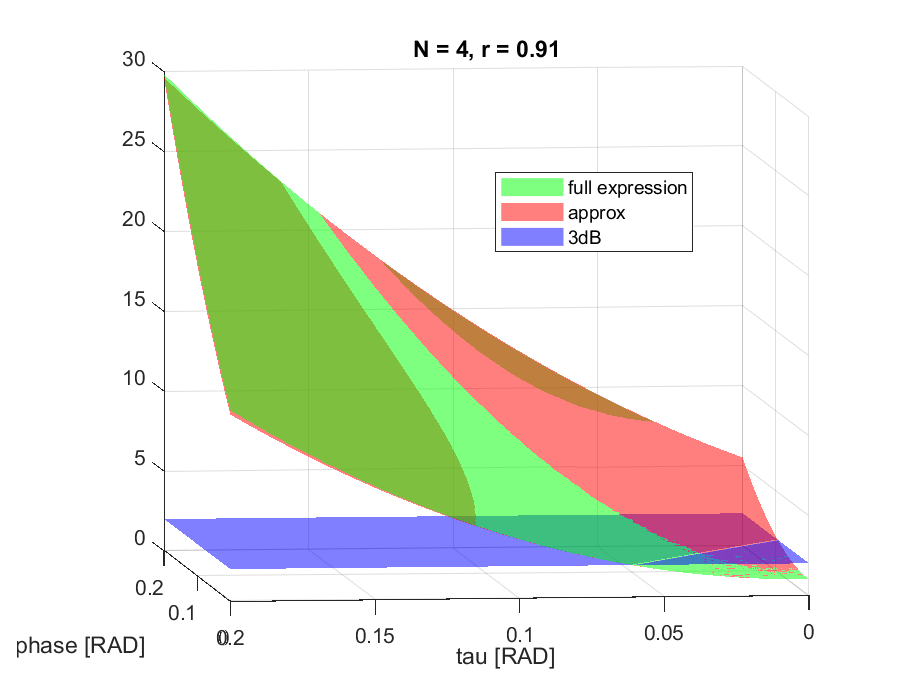
\includegraphics[width=0.9\linewidth]{./Media/spatial_IIR_MATLAB/beamwidth/BW_approx_validation.eps}
    \caption{Graphically comparing (\ref{eqn_arrayPerformance_beamwidth_fullEpxr}) and (\ref{eqn_arrayPerformance_beamwidth_approx}) for $N=4$ and $\rho=0.91$. The approximation seems to closely match the original expression.}
\end{figure}
Unlike the passive ULA case, it is evident from figure (\ref{fig_singleFreqFeedback_2ndTaylorNumericalValidation}) that the $4^{th}$ order terms are not needed for the evaluation of $\theta_{HPBW}$. In perfect phase alignment (i.e. $\Delta_{\tau}=0$), the u-space expression for the HPBW is $$u_{HPBW} =
\frac{
\left|1-\rho\right|
}{
\pi{d}
}
\lambda
\sqrt{\frac{
12
}{
\left(N-1\right)\left(\left(1+2r\right)N-4r+1\right)
}}.
$$
Comparing to the classic ULA beamwidth \cite{VanTrees2002DetectionIV}, thoroughly discussed in appendix \ref{appendix_theULABeamwidth}, we can express the improvement factor as
$$
\frac{
0.89\frac{\lambda}{ND}
}{
\theta_{HPBW,IIR}
}
=
\frac{0.89}{\left|1-\rho\right|}\sqrt{\frac{1+2r}{12}}
$$
\todo{TODO}
\textbf{Add graph of the improvement factor}
% \subsection{The pole-based design approach}
% In this approach, we look for setting the response "poles" which minimize the denominator, thus maximizing the overall response magnitude. To evaluate the beamwidth, we chose to allocate all of the system's poles in a single position such that 
% $
% 1-\vecnot{\beta}^{T}\vecnot{d}_{\theta}e^{-j\tau}
% =
% \left(e^{j\theta}-re^{j\theta_{s}}\right)^{N}
% $
% where $N$ is the number of array sensors and $r \in \left[0,1\right)$ enables us to avoid treatment of $\infty$-valued expressions. Next, we look for $\theta$ such that
% $
% \left|\frac{
% \frac
% {
% \vecnot{\alpha}^{T}\vecnot{d}_{\theta_{s}}
% }{
% \vecnot{\beta}^{T}\vecnot{d}_{\theta_{s}}
% }
% }{
% \frac
% {
% \vecnot{\alpha}^{T}\vecnot{d}_{\theta}
% }{
% \vecnot{\beta}^{T}\vecnot{d}_{\theta}
% }
% }\right|
% = \frac{1}{\sqrt{2}}
% $. Assuming that, like in classical IIR filter design theory, the numerator behaviour is significantly "slower" than the denominator's which results in $\vecnot{\alpha}^{T}\vecnot{d}_{\theta} 
% \approx
% \vecnot{\alpha}^{T}\vecnot{d}_{\theta_{s}}$ reults in
% \begin{align*}
%     \left|\frac{
%     \vecnot{\beta}^{T}\vecnot{d}_{\theta}
%     }{
%     \vecnot{\beta}^{T}\vecnot{d}_{\theta_{s}}
%     }\right|
%     &= \frac{1}{\sqrt{2}}
%     \\
%     \left|
%     \frac{
%     \left(e^{j\theta}-re^{j\theta}\right)^{N}
%     }{
%     \left(e^{j\theta}-re^{j\theta_{s}}\right)^{N}
%     }
%     \right|
%     &=
%     \left|
%     \frac{
%     \left(1-re^{j\left(\theta_{s}-\theta\right)}\right)
%     }{
%     \left(1-r\right)
%     }
%     \right|^{N}
%     \\
%     &=
%     \left|
%     \frac{
%     1+r^{2}-2r\cos{\left(\theta_{s}-\theta\right)}
%     }{
%     \left(1-r\right)^{2}
%     }
%     \right|^{\frac{N}{2}}
%     =
%     \left(\frac{1}{2}\right)^{\frac{1}{2}}
%     \\
%     \Rightarrow 
%     1+r^{2}-2r\cos{\left(\theta_{s}-\theta\right)}
%     &=
%     \left(1-r\right)^{2}2^{\frac{1}{N}}
%     \\
%     \cos{\left(\theta_{s}-\theta\right)}
%     &=
%     \frac{
%     1+r^{2}-\left(1-r\right)^{2}2^{\frac{1}{N}}
%     }{
%     2r
%     }
%     \\
%     \Rightarrow
%     \frac{\omega{D\left(cos(\theta_{g,s})-cos(\theta_{g,B})\right)}}{c}
%     &=
%     cos^{-1}
%     \left(
%     \frac{1+r^{2}-\left(1-r\right)^{2}2^{\frac{1}{N}}}{2r}
%     \right)
% \end{align*}.
% Therefore,
% \begin{equation}
%     \theta_{g,B} 
%     &= 
%     cos^{-1}
%     \left(
%     cos(\theta_{g,s})
%     -
%     \frac{c}{\omega{D}}
%     cos^{-1}
%     \left(
%     \frac{1+r^{2}-\left(1-r\right)^{2}2^{\frac{1}{N}}}{2r}
%     \right)
%     \right)
% \end{equation}
% Few observations can be derived from the $ \theta_{g,B} $:
% \begin{itemize}
%     \item $r\rightarrow{1}$ (i.e. setting the pole on the unit circle) causes $\theta_{g,B}\rightarrow\theta_{g,s}$ due to the $\infty$ valued response at $\theta_{g,s}$
%     \item The interval 
%     $
%     \left\{
%     \theta_{g,s}
%     \ \Bigg{|}\ 
%     cos(\theta_{g,s})
%     -
%     \frac{c}{\omega{D}}
%     cos^{-1}
%     \left(
%     \frac{1+r^{2}-\left(1-r\right)^{2}2^{\frac{1}{N}}}{2r}
%     \right)
%     <-1
%     \right\}
%     $, has no solution. In simulations, when evaluating such $\theta_{g,s}$ values, one can observe that the actual beampattern does not resemble the designed one due to the ULA geometric properties.
%     \item The number of sensors $N$ seems to have low impact on the beamwidth.
% \end{itemize}
\subsection*{Sidelobes attenuation}
\ifdefined\showDev
    \fbox{
    \begin{minipage}{0.9\linewidth}
    \textbf{development specifics}\\
    Let $f\rBrace{\dTheta} \triangleq \D{\dTheta/2}{N}\exp\rBrace{-j\rBrace{(N-1)\dTheta/2}},$ such that $\Hr_{\Delta\theta,\Delta\phi=0,r=0}\omegaB = \frac{f\rBrace{\dTheta}}{1-rf\rBrace{\dTheta}}.$ Then, we compute the beampattern's derivative and state that
    \begin{equation*}
    % \resizebox{0.9\linewidth}{!}{
        \begin{split}
            &\frac{\partial}{\partial\dTheta}\Hr_{\Delta\theta,\Delta\phi=0,r}\omegaB &\\
            &=\frac{\Dp{\dTheta/2,N}{'}\rBrace{1-r\D{\dTheta/2}{N}}-\D{\dTheta/2}{N}\rBrace{-r\Dp{\dTheta/2,N}{'}}}{\rBrace{1-r\D{\dTheta/2}{N}}^{2}}
            \\
            &=\frac{\Dp{\dTheta/2,N}{'}}{\rBrace{1-r\D{\dTheta/2}{N}}^{2}}.
        \end{split}
        % }
    \end{equation*}
    It follows that the sidelobes of the feedback based beampattern are located at the same angles as the in the ULA case.
    \end{minipage}
    }
\else
\fi
By taking a derivative of $\Hr_{\Delta\theta,\Delta\phi=0,r=0}\omegaB$ with respect to $\dTheta$ it can be easily verified that the beampattern's extrema points are located exactly as in the standard ULA beampattern. Specifically, the sidelobes locations are
\begin{equation}
    \label{eqn_CB_sidelobesLocations}
    \Delta\theta_{\text{sidelobe}} = \frac{\rBrace{2m+1}\pi}{N}\ \forall m\in\cBrace{\pm 1,\pm 2,\hdots}.
\end{equation}
Our main interest is with the first sidelobe (i.e. $m=1$), therefore we evaluate \eqref{eq_Hdphi0} at $\Delta\theta = 3\pi/N$, which results in
\begin{equation}
    \abs{\Hr_{{3\pi}/{N},0,r}\omegaB}^2
    =
    \frac{
    2\rBrace{1-r}^{2}
    }{
    \rBrace{N^{2}-2Nr}\rBrace{1-\cos{\rBrace{\frac{3\pi}{N}}}}+2r^{2}
    }
    \label{eq_HSidelobes}
\end{equation}
and for large $N$ values 
\begin{equation*}
    \lim_{N\rightarrow\infty}\abs{\Hr_{3\pi/N,0,r}\omegaB}=\frac{
    2\rBrace{1-r}
    }{
    3\pi
    }.
\end{equation*}
\ifdefined\showDev
    \fbox{
    \begin{minipage}{0.9\linewidth}
    \textbf{development specifics}\\
    We know that \eqref{eq_Hdphi0} can be rewritten as
    \begin{equation*}
        \begin{split}
            \Hr_{\Delta\theta,\Delta\phi=0,r=0} \omegaB=
            \frac{
            \rBrace{1-\cos{\rBrace{N\dTheta}}}\rBrace{1-r}^{2}
            }{
            \begin{split}
                N^{2}&\rBrace{1-\cos{\dTheta}}+r^{2}\rBrace{1-\cos{N\dTheta}}
                \\
                &+Nr\Bigg(1+\cos{\rBrace{\rBrace{N-1}\dTheta}}
                \\
                &-\cos{\rBrace{N\dTheta}-\cos{\rBrace{\dTheta}}}\Bigg)
            \end{split}
            }
        \end{split}
    \end{equation*}
    Using the symbolic toolbox in MATLAB, setting $\dTheta=3\pi/N$, results in \eqref{eq_HSidelobes}.
    \end{minipage}
    }
\else
\fi
\par For standard ULA, the gain of the first sidelobe is known to be $\frac{2}{3\pi}$ \cite{van2004optimum}, which implies that the suggested feedback based system has a suppression improvement of $1/\rBrace{1-r}$ at the first sidelobe.
Specifically, in perfect gain match (i.e. $r\to{}1$) scenario, the sidelobes vanish. 
\subsection*{Array directivity}
The array directivity $\mathcal{D}$ \cite{van2004optimum}, defined as
\begin{equation}\label{eq_D}
    \mathcal{D}\rBrace{N,r} = \frac{\Hr_{\Delta\theta=0,\Delta\phi=0,r}}{\frac{1}{2\pi}\int_{0}^{2\pi}\Hr_{\Delta\theta,\Delta\phi=0,r}\ d\Delta\theta} = \frac{2\pi}{\int_{0}^{2\pi}\Hr_{\Delta\theta,\Delta\phi=0,r}\ d\Delta\theta},
\end{equation}
measures the ratio between the maximal array gain at its mainlobe, to the averaged gain over all directions. 
For uniformly weighted ULAs with no feedback, it is known \cite{van2004optimum} that $\mathcal{D}\rBrace{N,0} = N$.
Plugging \eqref{eq_Hdphi0} within \eqref{eq_D}, combined with the use of numerical integration methods, we find that (see Fig.~\ref{fig_directivity})
\begin{equation}\label{eq_D}
    \mathcal{D}\rBrace{N,r} = \frac{N-r}{1-r}.
\end{equation}
\begin{figure}[t]
    \begin{center}
        \begin{overpic}[width=0.75\linewidth, 
        %grid, 
        tics=10,trim=0 0 0 0]{./Media/directivity_expr.eps}
            \put (20, 10){\footnotesize{$N$}}
            \put (72, 6){\footnotesize{$r$}}
            \put (16.5, 70){\footnotesize{Numerical integration}}
            \put (16.5, 65){\footnotesize{$\rBrace{N-r}/\rBrace{1-r}$}}
            \put (-9, 45){\footnotesize{$\mathcal{D}\rBrace{N,r}$}}
        \end{overpic}
    \end{center}
     \caption{Plot of $\mathcal{D}\rBrace{N,r}$, computed using numerical integration (surface), shown to perfectly match the analytic expression (black diamonds) presented in \eqref{eq_D}.}
    \label{fig_directivity}
\end{figure}
Note that the standard ULA's known result is obtained for $r=0$.
Also, for $N>=2$, $\lim_{r\rightarrow 1}\mathcal{D}\rBrace{N,r}=\infty$, implying infinite directivity for the perfectly gain matched FB. 
\par Finally, expressing the improvement in directivity compared to the standard ULA, assuming large $N$ values, gives rise to
\begin{equation}\label{eq_Dimprovement}
\frac{\mathcal{D}\rBrace{N,r}}{\mathcal{D}\rBrace{N,0}}\overset{N\gg1}{\approx}\frac{N/\rBrace{1-r}}{N}=\frac{1}{1-r}.
\end{equation}
\subsection*{Summary}
To conclude this section, we summarize the feedback integration related performance improvements in Table.~\ref{table_arrayPerformance} 
\begin{table}[h!]
    \centering
    \resizebox{1\linewidth}{!}{
        \begin{tabular}{||c c c c||} 
            \hline
            & ULA & \thead{FEEDBACK\\BASED} & IMPROVEMENT \\ [0.5ex] 
            \hline\hline
            HPBW & $ 1.4/N$ & $1.4/\rBrace{f(r)N}$ & $f\rBrace{r}$ times smaller\\ 
            \thead{FIRST\\SIDELOBE\\GAIN} & $2/3\pi$ & $2\rBrace{1-r}/3\pi$ & \thead{$1/\rBrace{1-r}$ times lower\\for $N\gg{}1$} \\
            DIRECTIVITY & $N$ & $\rBrace{N-r}/\rBrace{1-r}$ & \thead{$1/\rBrace{1-r}$ time higher \\ for $N\gg{}1$}\\
            [1ex] 
            \hline
         \end{tabular}
     }
    \caption{Comparing performances of classical ULA and the proposed feedback based architecture, with gain mismatch $r$.}
    \label{table_arrayPerformance}
\end{table}